\documentclass[10pt,a4paper,oneside]{article}
\usepackage{cmap}
\usepackage[T2A]{fontenc}
\usepackage{float}
\usepackage{listings}
\usepackage{csquotes}
\usepackage[utf8]{inputenc}
\usepackage{amsmath}
\usepackage{amsfonts}
\usepackage{amssymb}
\usepackage[english, russian]{babel}%Подключаем русский язык.
\usepackage{graphicx}
\usepackage{geometry} % Меняем поля страницы.
\geometry{left=3cm} %Левое поле.
\geometry{right=2cm} %Правое поле.
\geometry{top=3cm} %Верхнее поле.
\geometry{bottom=2cm} %Нижнее поле.


%Начало документа
\begin{document}

%Создаём титульник.
\begin{titlepage}
\newpage
	%Название ВУЗа и институт.
	\begin{center}
		\Large Санкт-Петербургский Государственный Политехнический Университет\\
		Институт Компьютерных Наук и Технологий\\
	\end{center}
	%Кафедра.
	\begin{center}
		\large\textbf {Высшая школа интеллектуальных систем и суперкомпьютерных технологий}
	\end{center}
	
	%Пропуск места. 
	\vspace{5em}
	%!!!!!!!!!!!!!!!!!!!!!!!!!!!!!!!!!Название работы.
	\begin{center}
		\large{Отчёт по лабораторной работе №3 \\ на тему \\
		\textbf{Апериодические сигналы} }
	\end{center}
	
	%Делаем пропуск и пишем студента и преподавателя.
	\vspace{25em}
	\begin{flushright}
		\textbf{Работу выполнил\\}Студент группы 3530901/80203 \\ Тарасенко Н.С.\\
		\textbf{Преподаватель\\}Богач Н.В. 
	\end{flushright}
	
	\vspace{\fill}%В самом низу
	\begin{center}
	Санкт-Петербург, 2021 год	
	\end{center}
\end{titlepage} %Закончили титульный лист.

\section{Настройка проекта}
Перед тем как выполнять задания необходимо настроить проект и сделать все необходимые импорты:

\begin{figure}[H]
        \centering
        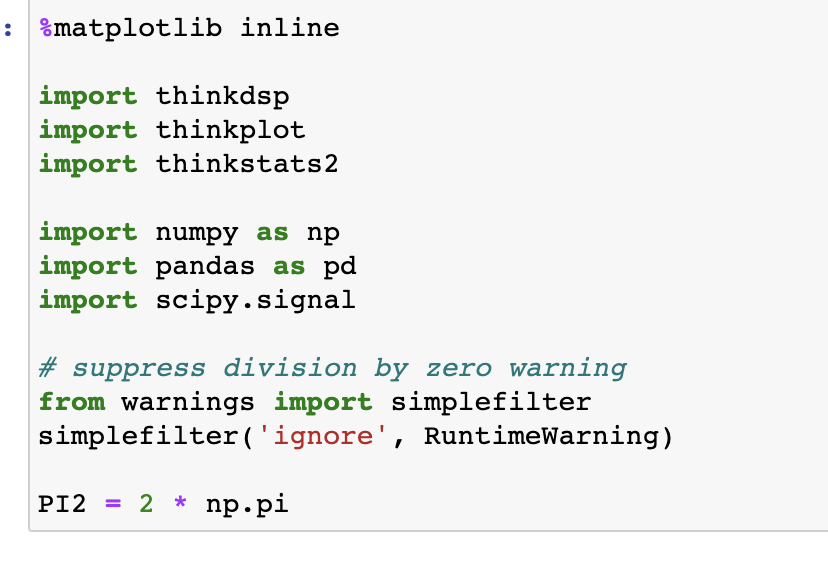
\includegraphics[width=0.75\textwidth]{0.png}
        \caption{2}
        \label{fig:first}
\end{figure}

\section{Упражнение номер №1}

Необходимо посмотреть пример утечки и заменить окно Хэмминга одним из окон предоставляемых numPy, посмотреть, как они влияют на утечку. 

Рассмотрим пример утечки, выведем его спектр: 

\begin{figure}[H]
        \centering
        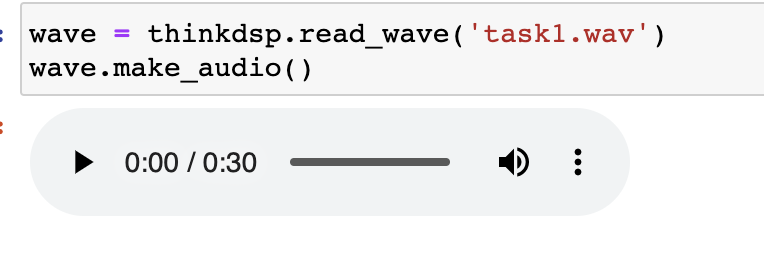
\includegraphics[width=0.75\textwidth]{1.png}
        \caption{2}
        \label{fig:first}
\end{figure}

Сделаем представление ввиде других 4 окон и наложим полученные спектры: 

\begin{figure}[H]
        \centering
        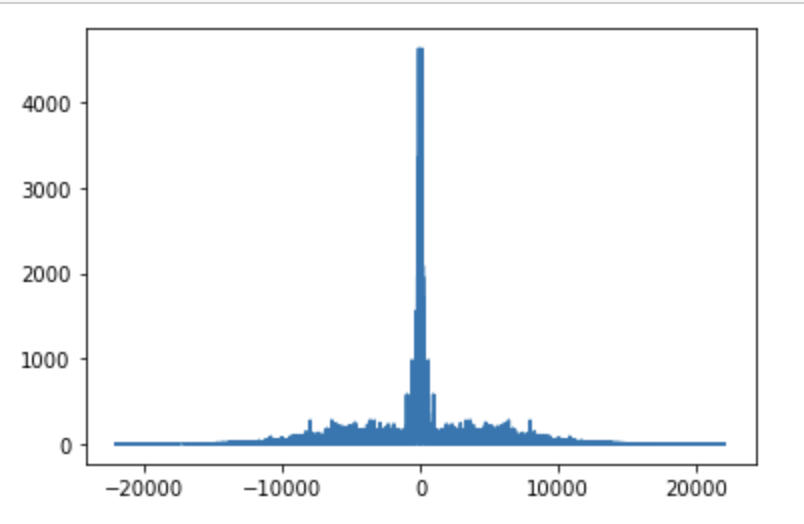
\includegraphics[width=0.75\textwidth]{2.png}
        \caption{2}
        \label{fig:first}
\end{figure}

Все четыре хорошо справляются с уменьшением утечки. Фильтр Бартлетта оставляет некоторый остаточный «звон». Фильтр Хэмминга рассеивает наименьшее количество энергии.

\section{Упражнение номер №2}

1) Необходимо создать класс SawtoothChirp, расширяющий Chirp и переопределяющий evaluate для генерации пилообразного сигнала с линейно увеличивающийся/уменьшающейся частотой.
2) Необходимо нарисовать эскиз спектрограммы этого сигнала и распечатать его. Попытаться услышать эффект биения

Реализуем класс SawtoothChirp

\begin{figure}[H]
        \centering
        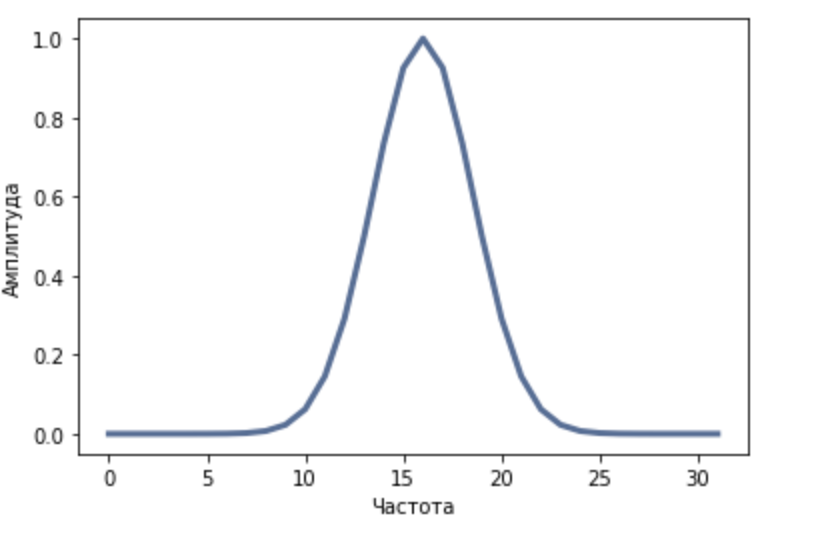
\includegraphics[width=0.75\textwidth]{3.png}
        \caption{2}
        \label{fig:first}
\end{figure}

Используя класс, который мы реализовали, создадим звук: 

\begin{figure}[H]
        \centering
        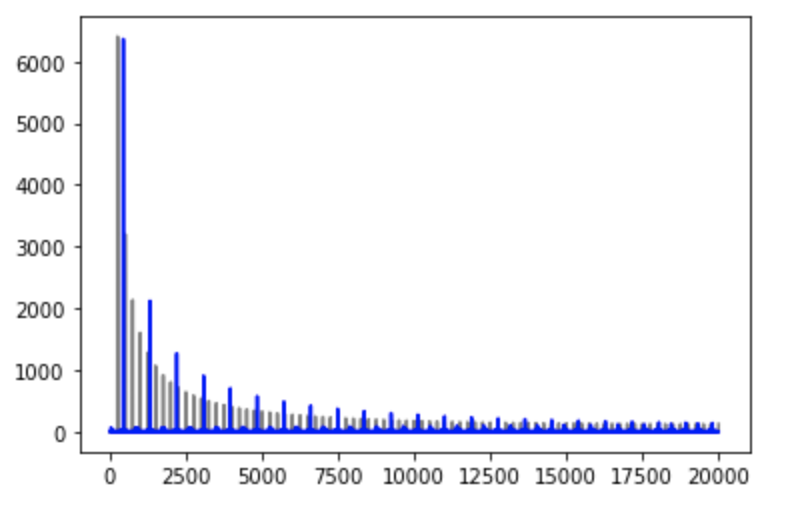
\includegraphics[width=0.75\textwidth]{4.png}
        \caption{2}
        \label{fig:first}
\end{figure}

Распечатаем спектрограмму получившегося звука: 

\begin{figure}[H]
        \centering
        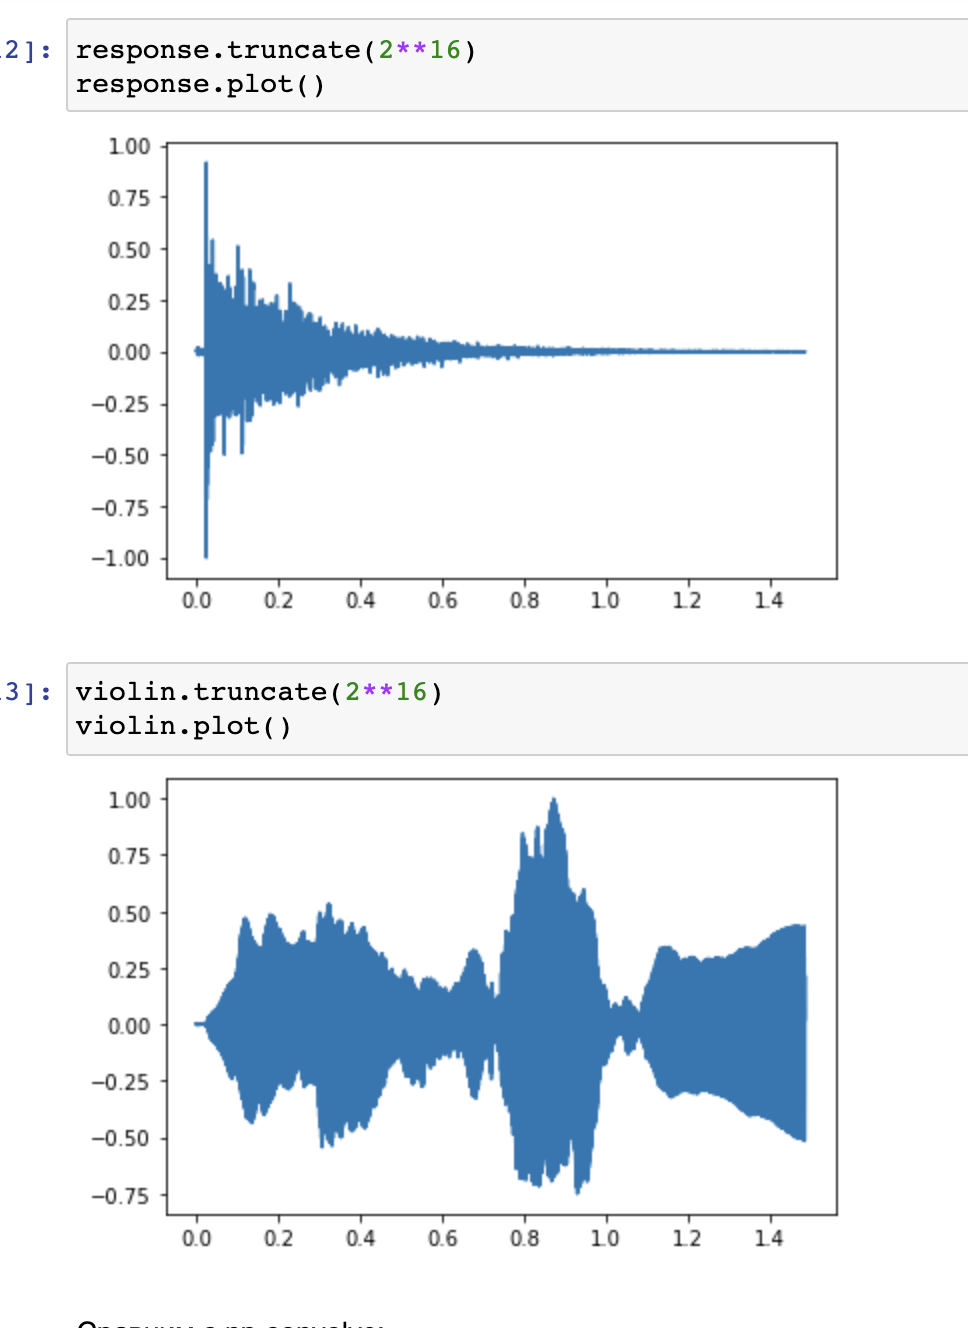
\includegraphics[width=0.75\textwidth]{5.png}
        \caption{2}
        \label{fig:first}
\end{figure}

При относительно низкой частоте кадров вы можете увидеть, как гармоники с наложенными частотами отражаются от частоты сворачивания.

\section{Упражнение номер №3}

Необходимо создать пилообразный чирп, меняющийся от 2500 до 3000 Гц, и на его основе сгенерировать сигнал длительностью 1с и частотой кадров 20кГц. Распечатать спектр.

Поскольку основная частота колеблется от 2500 до 3000 Гц, мы ожидаем увижеть всплеск. Первая гармоника колеблется от 5000 до 6000 Гц, поэтому в даннос случае всплеск будет меньше чем в первом случае. Следующая гармоника колеблется от 7500 до 9000 значит всплеск будет еще меньше чем во 2 случае.

Другие гармоники повсюду накладываются друг на друга, и образуют энергию. Эта распределенная энергия создает интересные звуки.

\begin{figure}[H]
        \centering
        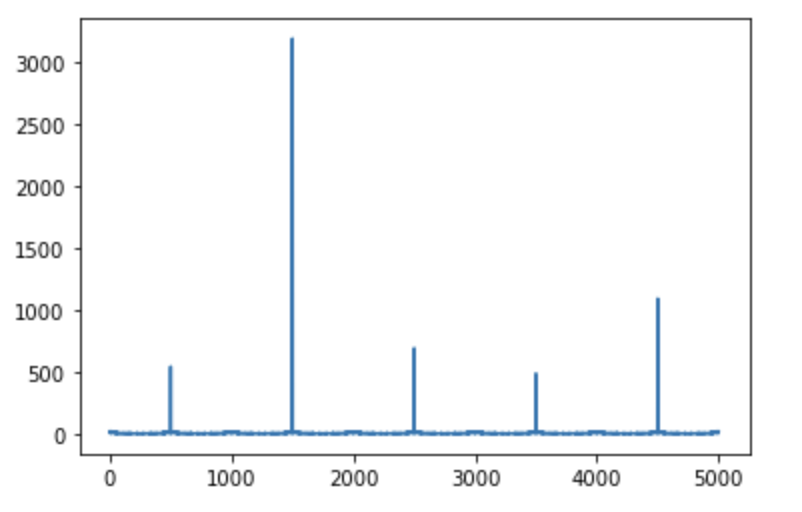
\includegraphics[width=0.75\textwidth]{6.png}
        \caption{2}
        \label{fig:first}
\end{figure}
 
 Распечатаем получившийся спектр: 
 
\begin{figure}[H]
        \centering
        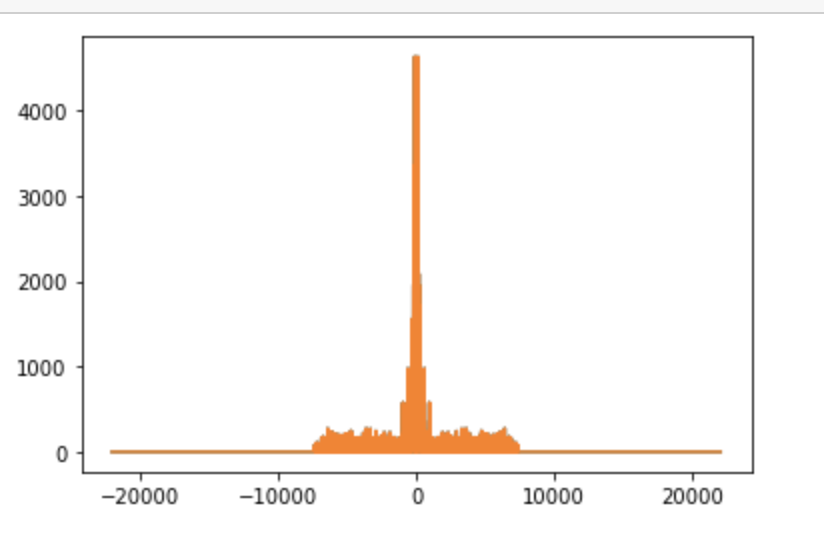
\includegraphics[width=0.75\textwidth]{7.png}
        \caption{2}
        \label{fig:first}
\end{figure}

\section{Упражнение номер №4}

Необходимо найти или записать звук глиссандо и распечатать спектрограмму первых нескольких секунд:

Для этого упражнения я взял звук из данного нам репозитория и обрезал его до первых 11 секунд: 

\begin{figure}[H]
        \centering
        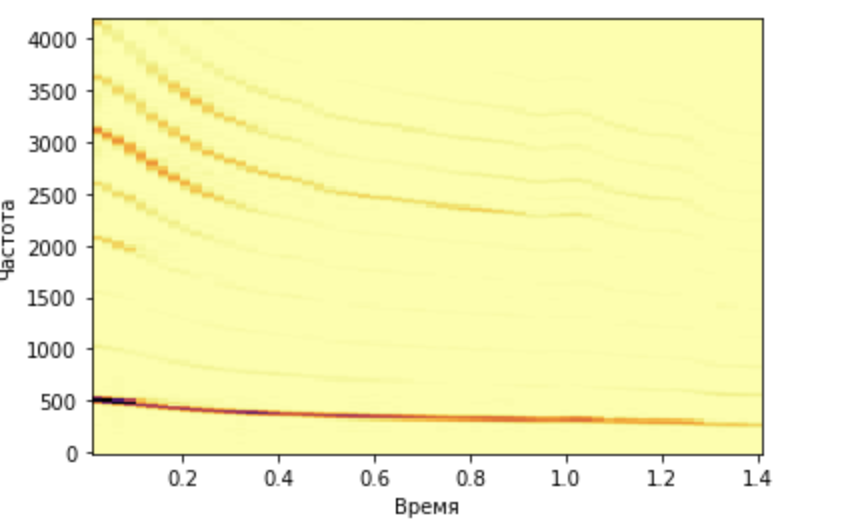
\includegraphics[width=0.75\textwidth]{8.png}
        \caption{2}
        \label{fig:first}
\end{figure}

Рассмотрим спектрограмму: 

\begin{figure}[H]
        \centering
        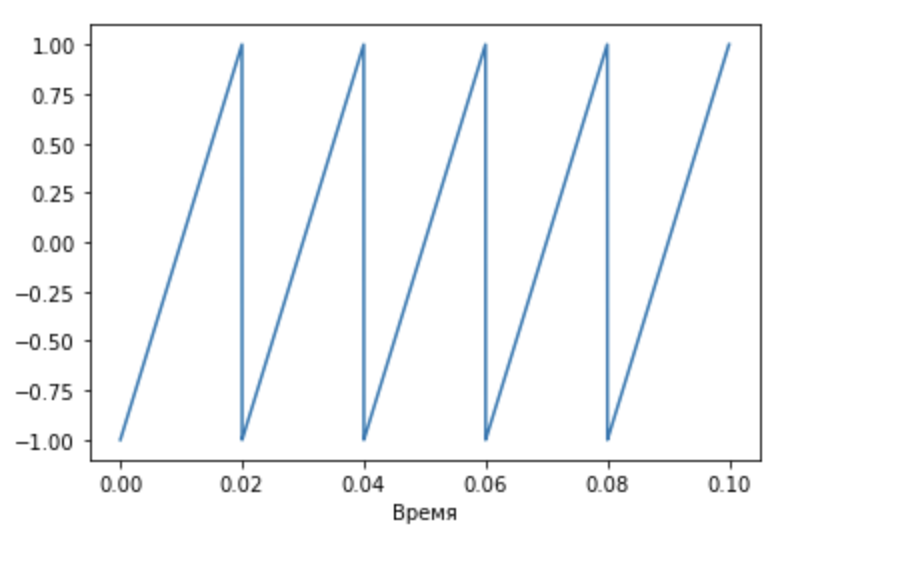
\includegraphics[width=0.75\textwidth]{9.png}
        \caption{2}
        \label{fig:first}
\end{figure}

\section{Упражнение номер №5}

Необходимо проанализировать как будет меняться во времени частота, при условии, что музыкант двигает кулису с постоянной скоростью. Необходимо реализовать класс TromboneGliss, расширяющий chirp и предоставляющий evaluate. Создать сигнал имитирующий глиссандо на тромбоне от C3 до F3, и обратно до C3. Распечатать спектрограмму полученного сигналаи определить на что похоже глиссандо на линейный или экспоненциальный чирп.

Реализуем наш класс, которы	 будет представлять из себя сигнал схожий с тромбоподобными, имеющий переменную частоту.

\begin{figure}[H]
        \centering
        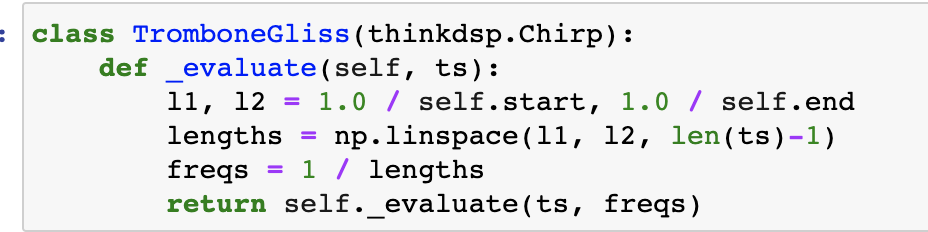
\includegraphics[width=0.75\textwidth]{10.png}
        \caption{2}
        \label{fig:first}
\end{figure}

Рассмотрим созданный нами сигнал , возьмем лишь первую его часть: 

\begin{figure}[H]
        \centering
        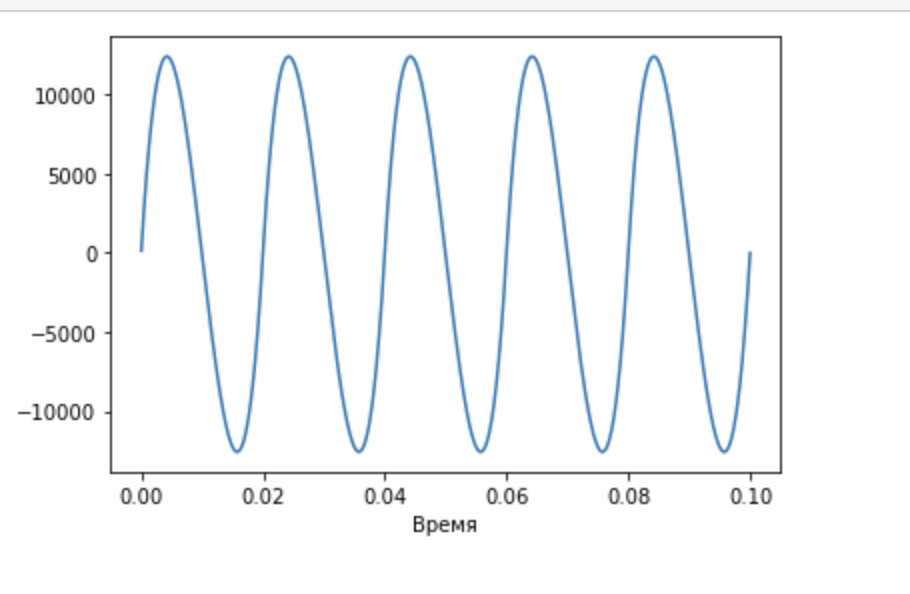
\includegraphics[width=0.75\textwidth]{11.png}
        \caption{2}
        \label{fig:first}
\end{figure}

Рассмотрим вторую часть сигнала: 

\begin{figure}[H]
        \centering
        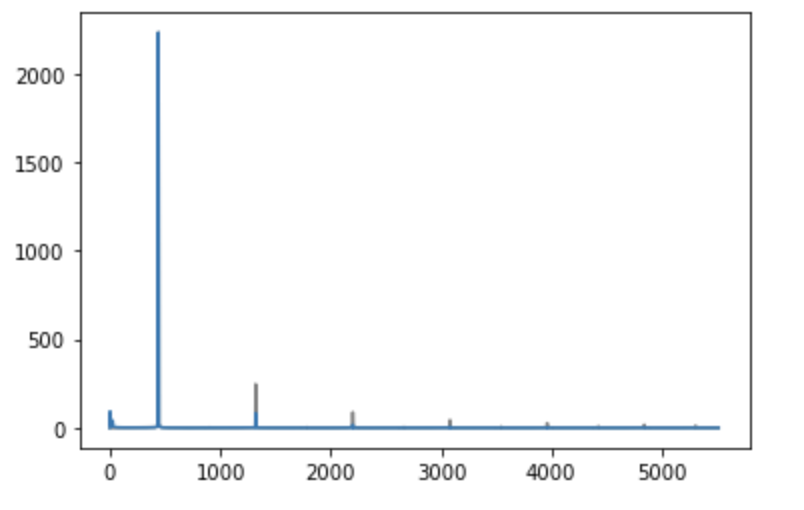
\includegraphics[width=0.75\textwidth]{12.png}
        \caption{2}
        \label{fig:first}
\end{figure}

И наконец соединим обе части и получим конечный результат: 

\begin{figure}[H]
        \centering
        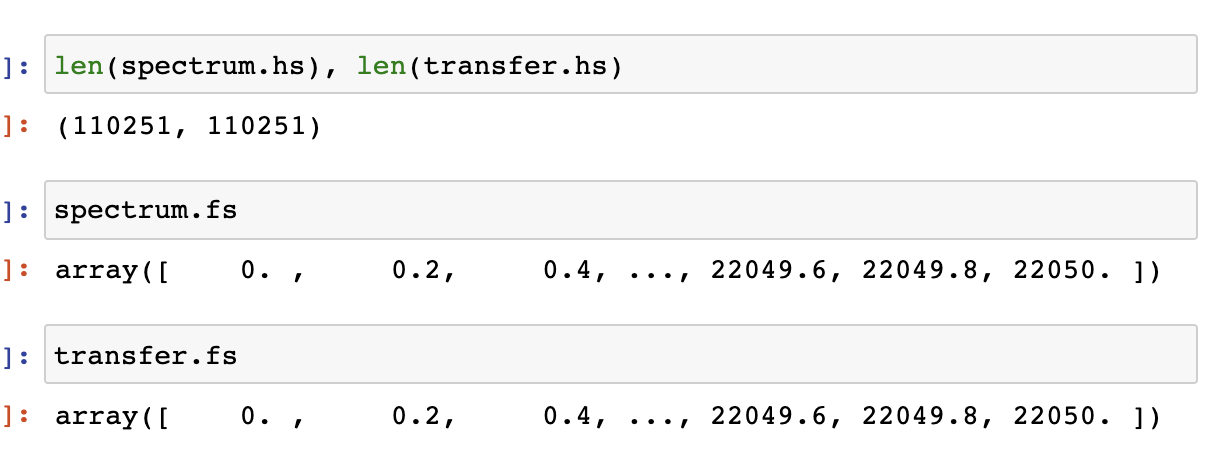
\includegraphics[width=0.75\textwidth]{13.png}
        \caption{2}
        \label{fig:first}
\end{figure}

Выведем спектрограмму: 

\begin{figure}[H]
        \centering
        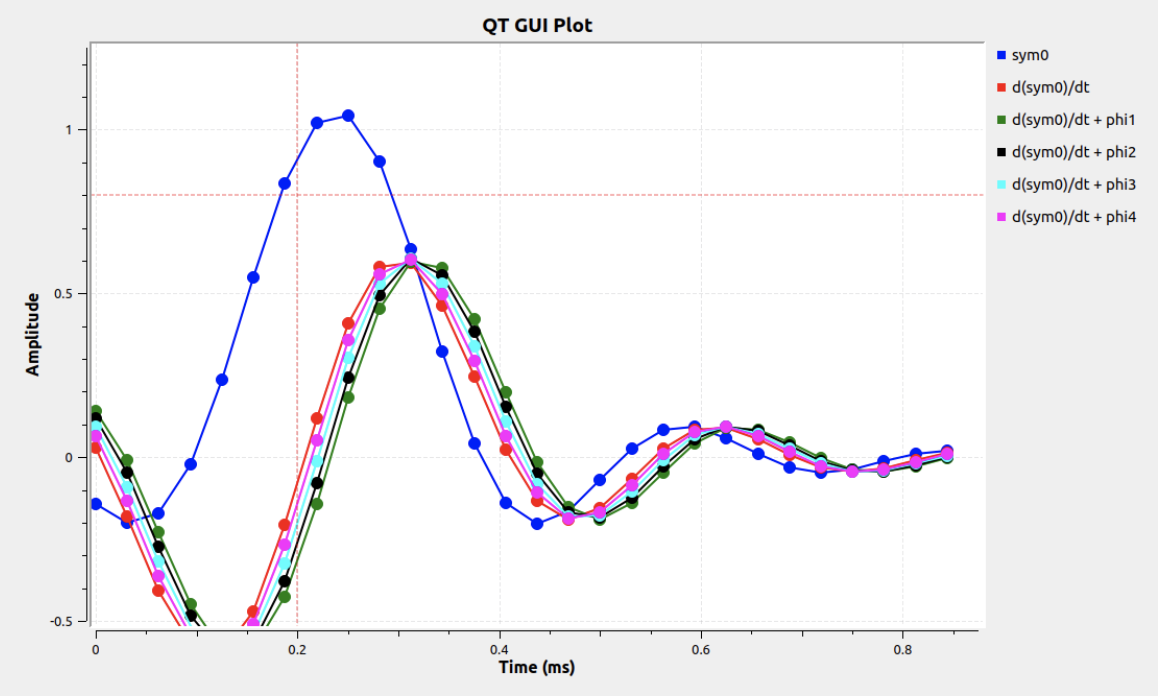
\includegraphics[width=0.75\textwidth]{14.png}
        \caption{2}
        \label{fig:first}
\end{figure}

Как видно из полученного графика и звуков, частота сначала возрастает, а потом снова уменьшается до начальной, следовательно, написанный класс работает корректно. К сожалению, с такой маленькой разницей в начальной и конечной частотах невозможно определить на что похоже глиссандо на тромбоне - на линейный или экспоненциальный чирп.

\section{Упражнение номер №6}

Для данного упражнения снова возьмем звук из предложенного нам репозитория. На нем мужчина произносит глассные звуки с эффектом "эхо"

\begin{figure}[H]
        \centering
        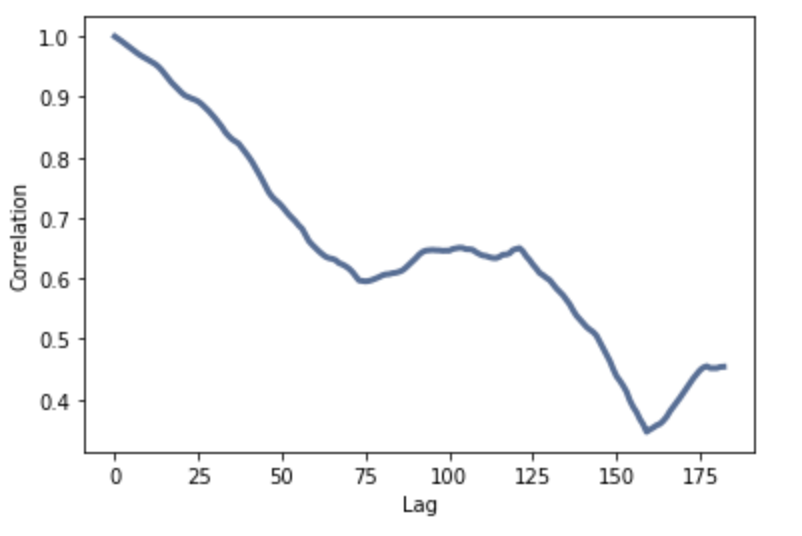
\includegraphics[width=0.75\textwidth]{15.png}
        \caption{2}
        \label{fig:first}
\end{figure}

Рассмотрим спектрограмму данного звука: 

\begin{figure}[H]
        \centering
        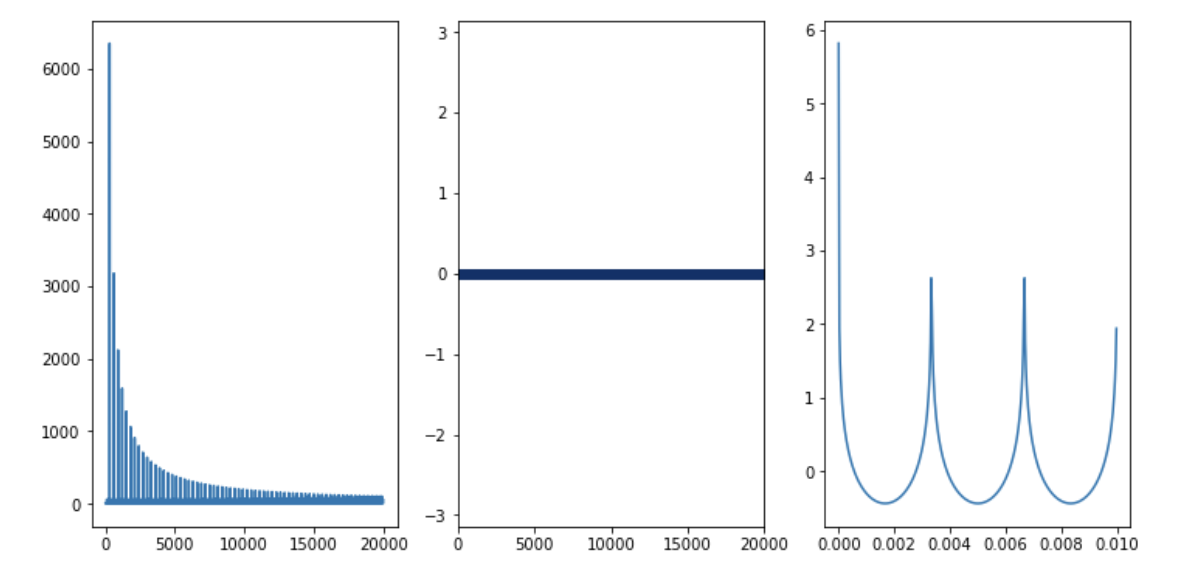
\includegraphics[width=0.75\textwidth]{16.png}
        \caption{2}
        \label{fig:first}
\end{figure}

Полоса внизу, вероятно, является фоновым шумом. Пики на спектрограмме называются формантами.

Распечатаем спектр, выделив сегмент во время "а":

\begin{figure}[H]
        \centering
        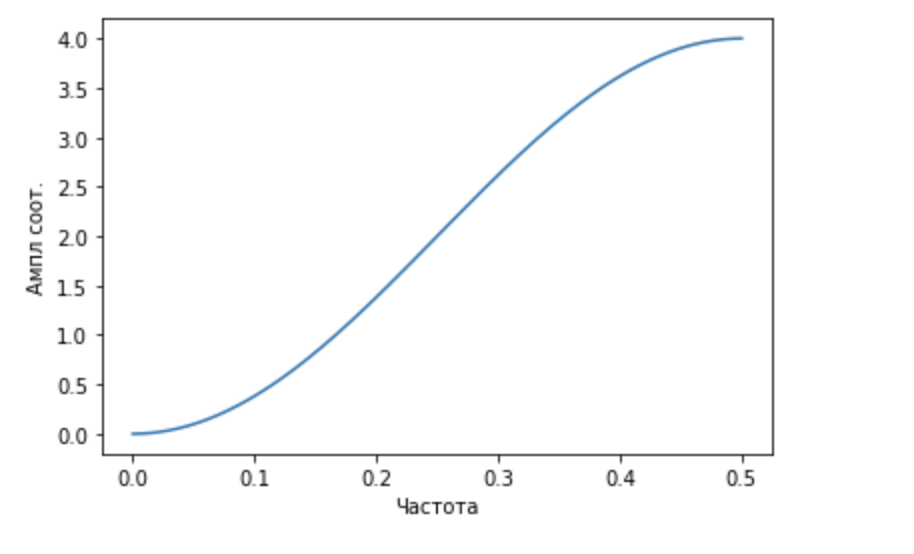
\includegraphics[width=0.75\textwidth]{17.png}
        \caption{2}
        \label{fig:first}
\end{figure}

Мы можем увидеть форматы уже более четче.

Выведем спектры и для остальных звуков: 

\begin{figure}[H]
        \centering
        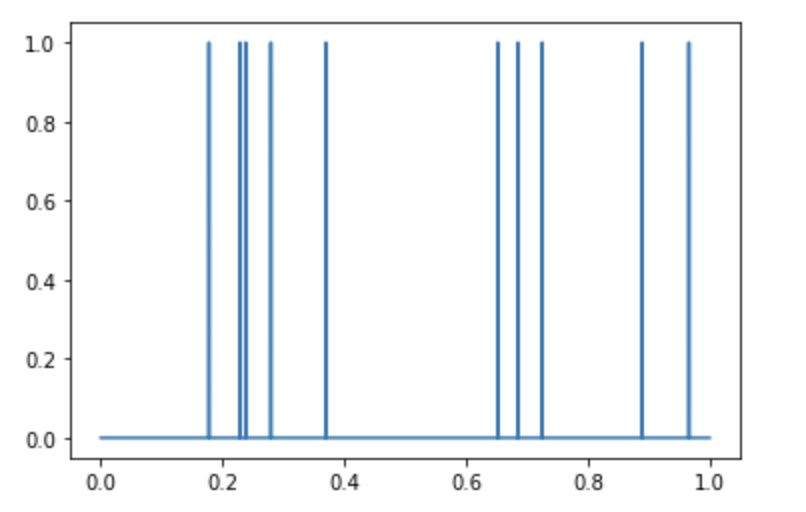
\includegraphics[width=0.75\textwidth]{18.png}
        \caption{2}
        \label{fig:first}
\end{figure}

Сегмент «э» имеет высокоамплитудную форманту около 500 Гц.

\begin{figure}[H]
        \centering
        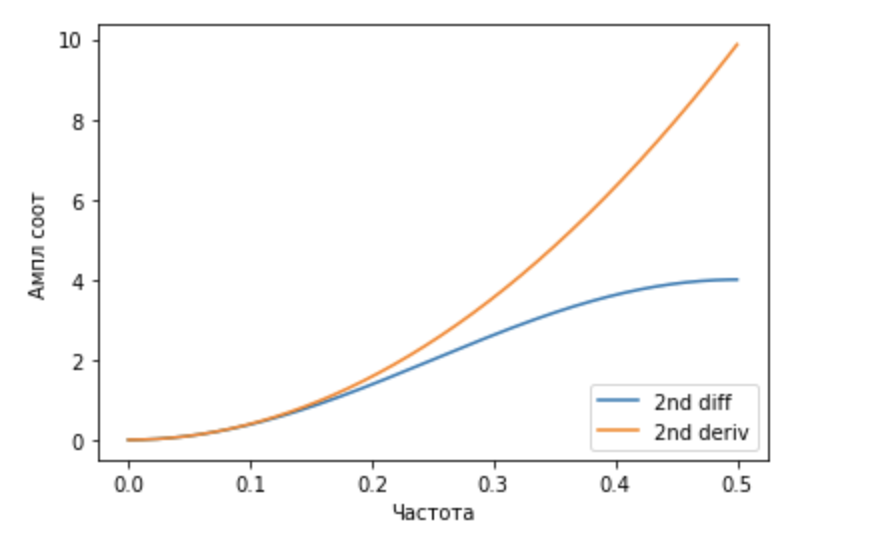
\includegraphics[width=0.75\textwidth]{19.png}
        \caption{2}
        \label{fig:first}
\end{figure}

В сегменте "и" нет высокочастотных составляющих.

\begin{figure}[H]
        \centering
        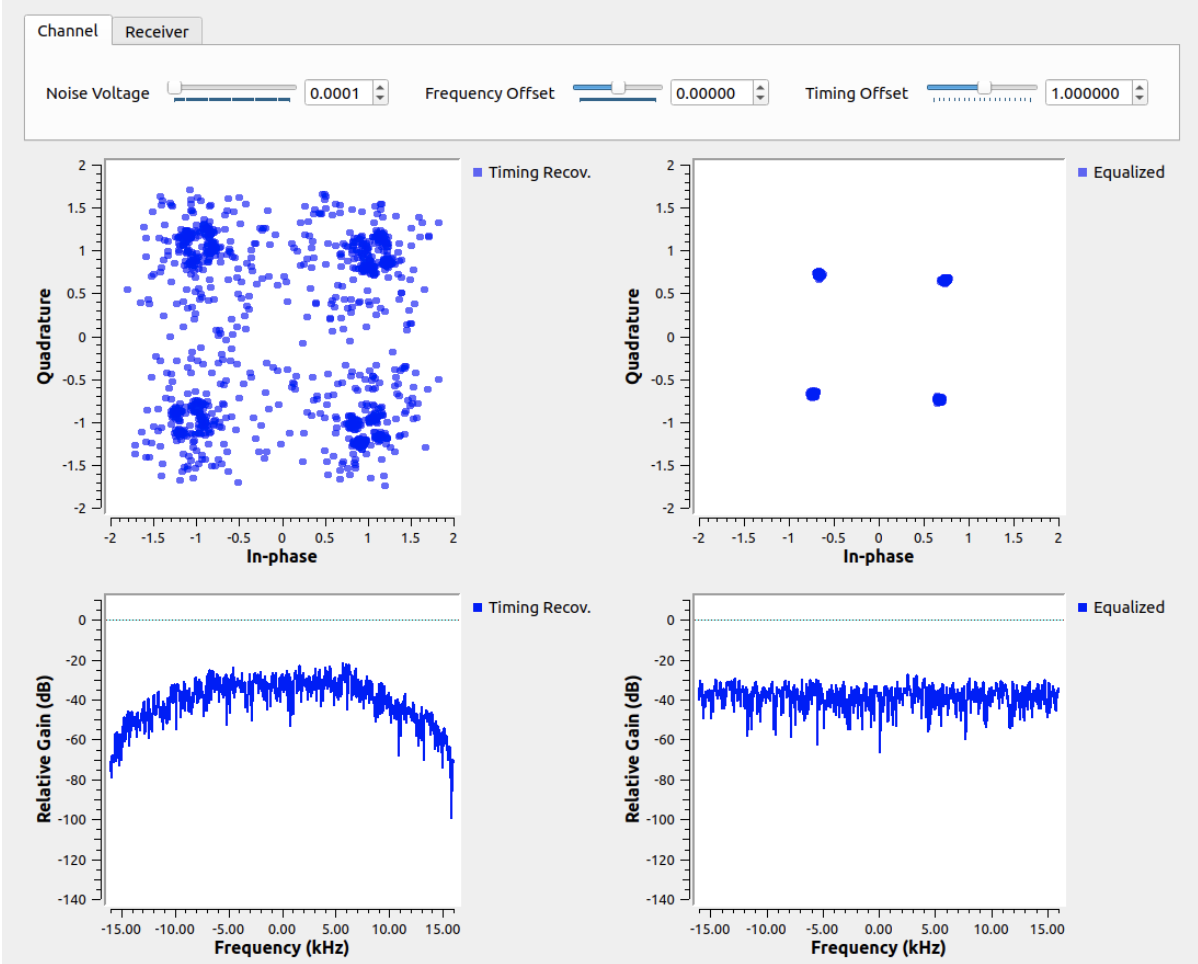
\includegraphics[width=0.75\textwidth]{20.png}
        \caption{2}
        \label{fig:first}
\end{figure}

Сегмент «о» имеет высокоамплитудную форманту около 500 Гц, даже выше основной гармоники.

\begin{figure}[H]
        \centering
        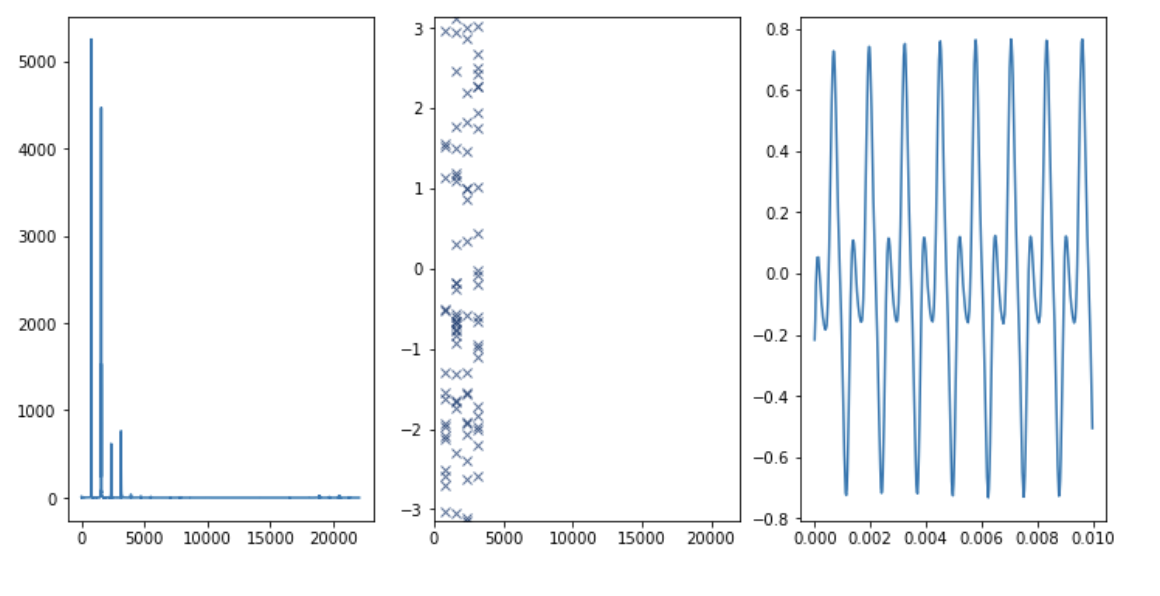
\includegraphics[width=0.75\textwidth]{21.png}
        \caption{2}
        \label{fig:first}
\end{figure}

Сегмент "у" имеет высокоамплитудную форманту около 300 Гц и не имеет высокочастотных составляющих.


\end{document}